\subsubsection{Satellite Data}

Copernicus stores data that is obtained from the usage of its 5 different \textbf{Sentinel Satellites}.
Each of these satellites collect different forms of data and all of this can be accessed through the Copernicus API
\begin{itemize}
    \item \textbf{Sentinel-1}, provides \underline{radar imagaging} that collects data that pertains to
    \begin{itemize}
        \item Landscape topography
        \item Multi-purpose imagery of both land and ocean
        \item Ocean Surface winds
        \item Ocean topography and currents
        \item Ocean wave height and spectrum
        \item Sea ice cover, edge and thickness
        \item Snow cover, edge and depth
        \item Soil moisture and vegetation
    \end{itemize}
    The following data is measured from S-1
    \begin{itemize}
        \item SAR (Synthetic Aperture Radar) transmits microwave signals at an angle and measures the backscatter echo. The brightness \underline{amplitude} and \underline{phase information} is being recorded. General variables that affect these measurements are
        \begin{itemize}
            \item Surface Roughness
            \item Dielectric constants of scattering material
        \end{itemize}
        \item Polarimetry, in which the \underline{polarization} of EM radiation is studied. Applications for polarimetric data are
        \begin{itemize}
            \item Crop identification, condition monitoring and soil moisture in agriculture
            \item Biomassn estimation, species identification and fire scar mapping in forestry
            \item Sea ice identification, coastal wind field measurements, oil spill detection in oceanography
        \end{itemize}
        \item Interferometry, measuring the \underline{phase difference} between two complex radar SAR observations from the same area. Applications of the interferometry are 
        \begin{itemize}
            \item Geophysical monitoring of natural hazards
            \item Time series analysis of surface deformations
            \item Glacier motion analysis
            \item Elevation mapping
        \end{itemize}
    \end{itemize}
    \item \textbf{Sentinel-2}, a pair of satellites that perform \underline{multi-spectral imagaging}. These satellites are phased at 180 degrees and samples at 13 different spectral bands. The spectral bands can be divided into 3 different groups based on their spatial resolution
    \begin{itemize}
        \item 10m resolution band that contains 4 different bands in the visible part of the EM spectrum
        \begin{itemize}
            \item Blue light ($\sim$493 nm)
            \item Green light ($\sim$560 nm)
            \item Red light ($\sim$665 nm)
            \item near IR light ($\sim$833 nm)
        \end{itemize}
        \begin{figure}[h!]
            \centering
            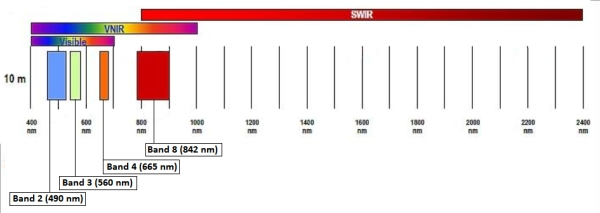
\includegraphics[width=\textwidth]{data_sources/img/sentinel2-bands1.png}
            \caption{Overview of the 10m spectral resolution band}
        \end{figure}
        \item 20m resolution band that contains 6 different bands mainly in the IR region of the EM spectrum
        \begin{itemize}
            \item 4 narrow bands in visible-near IR (vnIR) ($\sim$704nm,$\sim$740nm, $\sim$783nm and $\sim$865nm), aimed at vegetation detection
            \item 2 wider bands in shot-wave IR (swIR) ($\sim$1610nm and $\sim$2190nm) aimed at snow/ice/cloud detection or vegation moisture stress assessment
        \end{itemize}
        \begin{figure}[h!]
            \centering
            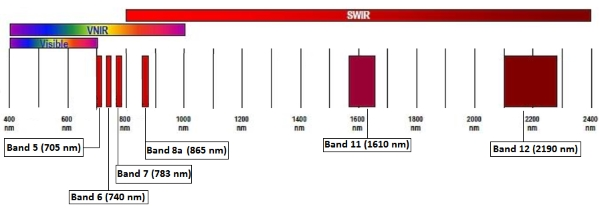
\includegraphics[width=\textwidth]{data_sources/img/sentinel2-bands2.png}
            \caption{Overview of the 20m spectral resolution band}
        \end{figure} 
        \item 60m resolution band that cointains 3 different bands that is focused on cloud screening and atmospheric correction ($\sim$443nm for aerosols and $\sim$945nm for water vapour) and cirrus detection ($\sim$1374nm)
        \begin{figure}[h!]
            \centering
            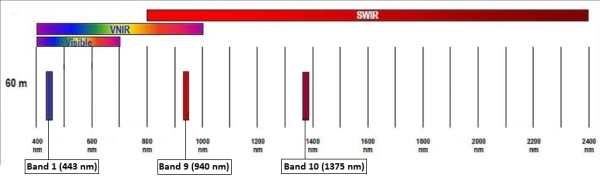
\includegraphics[width=\textwidth]{data_sources/img/sentinel2-bands3.png}
            \caption{Overview of the 60m spectral resolution band}
        \end{figure}
    \end{itemize}
\end{itemize}
